\documentclass[11pt,a4paper]{article}
\usepackage{cite,url,hyperref,graphicx, amsmath, bm}
\usepackage{alltt} 
\usepackage{listings}
\lstset{
basicstyle=\small\ttfamily,
columns=flexible,
breaklines=true
}



\setlength{\textwidth}{6.5in}
\setlength{\oddsidemargin}{0in}
\setlength{\evensidemargin}{0in}
\setlength{\topmargin}{-0.5in}
\setlength{\textheight}{25cm}
%opening
\title{Error Analysis of the Pairwise Sequentially Markovian Coalescent (PSMC) Model}
\author{Shaun D. Barker & Alex L. Jackson}
\begin{document}

\maketitle

%\begin{abstract}
%blah
%
%\end{abstract}
\section{Miscellaneous}
For further inquiries, I (Alex) can be contacted at \href{mailto:aj123@internode.on.net}{aj123@internode.on.net}.

If for some reason you can't get files from the dropbox, scripts and other things can be recovered from \url{https://github.com/alex-jackson1994/AlexBioProgs}, \url{https://github.com/alex-jackson1994/shaunScholarshipStuff} and \url{https://github.com/alex-jackson1994/ScholarshipSummary}. Apologies for the mess!

\section{Background Material}
\subsection{PSMC}
The Pairwise Sequentially Markovian Coalescent (PSMC) model \cite{li2011inference} is a method for estimating past population dynamics based on the  genome of a single individual. PSMC uses the heterozygousity of the genome to estimate where recombination events have occurred in the genome. These estimates are found using a Hidden Markov Model (for an introduction to HMMs, see the paper by Rabiner \cite{rabiner1989tutorial}). A genome is split into many consecutive, non-overlapping 100 bp ``bins''. The observations are whether each of the bins contains a heterozygous pair (``1''), is homozygous (``0''), or data is missing (``.''). The state space is the set of non-overlapping time intervals from the present back in time. The hidden state is the time interval into which the TMRCA for each bin falls. This allows PSMC to then construct a population estimate over a period of time. 

For further detail, see the paper by Li \cite{li2011inference} (the Methods section in particular gives a starting point) as well as the supplementary information for detail, and the package's README at \url{https://github.com/lh3/psmc}.

\subsection{File Types}
See the document \verb|fileTypes.pdf| for detail on the different file types (FASTA, FASTQ, SAM, BAM, MS, PSMCFA, PSMC).


\section{Methods}\label{sec:methods}
\subsection{Generating Simulated Data} %This almost falls under background material
We used genomic data simulated by msHOT-lite (\url{https://github.com/lh3/foreign/tree/master/msHOT-lite}) in our error analysis of the PSMC model. msHOT-lite is a modification by Li upon the genetic simulation software msHOT \cite{hellenthal2007mshot}, which is itself a modification upon the original software package ms \cite{hudson2002generating}. msHOT-lite allows us to simulate the genome of an individual subject to a specified number of base pairs, chromosomes, mutation rate, recombination rate and population history. 
An example of a msHOT-lite call is: 

\verb|msHOT-lite 2 1 -t 60000 -r 10000 1000000 -eN 1 2 -eN 2 4 -l >output.ms| 
This call simulates a diploid genome with a single chromosome (\verb|msHOT-lite 2 1|). Then \verb|-t 60000| sets the parameter $\theta$ to 60000 where $\theta=4N_0\mu$, where $\mu$ is the neutral mutation rate for the entire genome and $N_0$ is the initial population size. Then \verb|-r 10000 1000000| sets the parameter $\rho$ to 10000 and the number of base pairs per chromosome to 1000000 where $\rho=4N_0r$ and $r$ is the recombination probability per generation. Lastly \verb|-eN 1 2 -eN 2 4| introduces two population changes in the species history, firstly at time 1 (which is $4N_0$ generations ago) the population is set to 2 (which is $2\times4N_0$) and then at time 2 (which is $2\times4N_0$ generations ago) the population is set to 4 (which is $4\times4N_0$). The manual by Hudson \cite{hudson2002generating} provides further detail.

msHOT-lite can output several different formats. We used the \verb|-l| switch that outputs a text file containing a list of coordinates for heterozygous base pairs. We gave these the \verb|.ms| file extension. The \verb|-l| switch is very important - if it is not used, PSMC will not be able to run properly. The PSMC software package provides a Perl script called \verb|ms2psmcfa.pl|, which converts ms output into the \verb|.psmcfa| format that PSMC takes as an input. The file format \verb|.psmcfa| is FASTA-like. Each contig in the file is given a header line started by \verb|>|, and the sequence is recorded on 60 character long lines afterwards. Each character on these lines corresponds to a bin of 100 base pairs and shows whether at least one heterozygous base pair within that bin.

\subsection{Processing Real Data}
We took bison data from the ACAD server. The path for the bison reference genome is \verb|/localscratch/Refs/Bison_bison/Bos_taurus_BWA6_2_2015_08/Bison_UMD1_0.fasta| and the \verb|.bam| files required are in the folder \verb|/localscratch/jsoubrier/Bison_Genomes/BisonRef_MQ25|.

Working with real data requires a different approach to create the \verb|.psmcfa| PSMC input file. For our work we took a steppe bison genome in a binary alignment format (\verb|.bam|) file (the format of which was first described in \cite{li2009sequence}) as well as a reference bison genome as a FASTA (\verb|.fa|) file. The first step was to create a pseudo-diploid sequence in the FASTQ (\verb|.fq|) format from this data using the Samtools suite (we used version 1.3). This was accomplished using the following commands:
\begin{lstlisting}
samtools mpileup -EA -Q20 -C50 -u -f refBison.fasta SteppeBison.bam | bcftools call -c | vcfutils.pl vcf2fq | gzip > mpileupedSteppeBison.fq.gz
\end{lstlisting}
This command has four parts. Firstly, it performs a pileup where the steppe bison data is compared to the reference bison data. The pseudo-diploid sequence is then created\ using bcftools.  Then the output from that data is converted into FASTQ format using vcfutils. Finally, the whole thing is compressed using gzip. 

We call it pseudo-diploid as we are not finding hetero/homozygous sites by comparing chromosomal pairs. Instead, we compare the reference and the sequence, and differences between them are called heterozygous.

Once in this format we can use a utility provided with PSMC to create the \verb|.psmcfa| input file. PSMC includes the \verb|fq2psmcfa| script that converts compressed or uncompressed FASTQ format files into the required \verb|.psmcfa| input file.

Our \verb|pileupBAMFile.sh| script can be used to run the above set of commands, or they can just be typed in. If using the script, make sure you change the paths to samtools, bcftools and vcfutils, as well as the input variables. Samtools can be found at \url{https://github.com/samtools/samtools} and bcftools/vcfutils from \url{https://github.com/samtools/bcftools}.

\subsection{Data manipulation} 
Every PSMC run requires only a \verb|.psmcfa| input file. This is a convenient place where data can be modified efficiently for experiments. It is memory-efficient as each character represents 100 base pairs. Also, you can modify simulated or real data in the same way if it is converted to the \verb|.psmcfa| format.

\subsubsection{Splitting the Data}
The first experiment we considered was the effect of splitting the individual contigs into smaller contigs. This was accomplished using the Python script \verb|binarySplitPsmcfaPrint.py|. This script breaks each fragment in a \verb|.psmcfa| file into two equal length sequences. We did this recursively, taking a simulated genome and splitting it up until the genome contained many more sequences than it initially did. The minimum size for a split contig was set to 1 line (equivalent to 6 kbp).

% I have no idea what happened with this.
%\subsubsection{Combining the Data}
%The opposite of the previous section, we consider what would happen if we started joined every contig together into a single giant contig. This was achieved using the Bash script \verb|combinePsmcfa.sh|. 

\subsubsection{Deleting Data}
Another experiment we considered was deleting random data from the sequence. This was achieved using the Python script \verb|removeRandomPartsFromPsmcfa.py| which looped through the \verb|.psmcfa| file removing random lines from the file without deleting entire contigs. Physically a line in a \verb|.psmcfa| file represents 6000 base pairs, since a line is at most 60 characters long and each character is a bin of 100 base pairs. This was repeated, removing 10\%, 20\%, ... 90\% of the genome each time and running PSMC on the resulting smaller genomes using the Bash script \verb|partRemovalRepeated.sh|.



\subsubsection{Time Intervals}
Times in which a bin's TMRCA falls into is split up into discrete intervals, which can be specified in the input of the program. The intervals are split between the present and a maximum estimation time $T_{max}$ which is chosen by PSMC (for more detail, see the S.I. of Li \cite{li2011inference}). PSMC takes a pattern of intervals in the form of a string '$a$*$b$' where this would be $a$ intervals of length $b$. By default PSMC assumes a pattern of intervals '4+5*3+4' which is 4 intervals of length 1 followed by 5 intervals of length 3 followed by 4 intervals of length 1 again. For our experiments we ignored any intervals of length other than 1 and considered only splitting into equal length intervals of '10', '20', '30' and '40'.

%This is how I think it works: THESE ARE NOT ``REAL'' TIMES WHICH WE PLOT ON THE X AXIS OF OUR PSMC GRAPHS. The time intervals are where the TMRCAs fall into. Thus, for a '4+5*3+4' run, there would be 7 intervals, which I confirm in R.
%\begin{lstlisting}
%> unique(kanga1$pop_hist)
%[1] 2650.219 2824.702 1363.328 1216.244 1562.255 3080.304 7831.582
%\end{lstlisting}

% HOW IT WORKS: I'm not 100\% sure, but this is what I think. For example, let's say you ran PSMC with the interval parameters ``4+5*3+4''. This means that you've got 4 intervals of length 1, then 5 intervals of length 3, then 4 intervals of length 1. Intervals of length greater than 1 are made up of multiple atomic intervals, therefore the total number of intervals you have is $4+5\times3+4=23$. Meanwhile, while running PSMC, if you don't specify a \verb|-t| switch, the default maximum coalescent time ($T_\text{max}$ I think) is 15 (\verb|-t FLOAT    maximum 2N0 coalescent time [15]| from running the program without any input). This is on the $2N_0$ scale

\subsubsection{Contig Length in Real Data}\label{contigLength}
One difference between the simulated and the real data is the number of base pairs that are in each contig. Where simulated data has a constant number (specified in the \verb|ms| command), real data has a number of varied lengths per contig. The script \verb|summaryStatistics.py| takes a \verb|.psmcfa| file as an input and prints a tab delimited table of the minimum, maximum, median and of base pairs in each contig in the given file as well as the total number of base pairs in the entire file. We used these summary files when considering the effect of breaking up the data on the error.

\subsection{Running PSMC}
PSMC requires a \verb|.psmcfa| file as input can take several switches that modify default behaviour. We used the \verb|-p| switch to specify different time intervals as discussed above. For example, running PSMC using the following command
\begin{verbatim}
		./psmc -p '40*1' inputFile.psmcfa > outputFile.psmc
\end{verbatim}
performs PSMC on the given input file using 40 equal length time intervals. Run psmc without any input file to see further options.

\subsubsection{PSMC Output Files (.psmc)}
The output files generated by PSMC are a (roughly) tab delimited text format, where the first two characters on each line defines what values are on the line. The output files always contain a header which gives some information on the format, and then parameter estimates for each iteration of the Baum-Welch algorithm used in PSMC. The last table contains the estimates from the final iteration, this is the data we used for our analysis. The last table can be extracted as a tab delimited table using the script \verb|removeDataFromPSMC.sh|. This script takes a \verb|.psmc| output file as its input and then outputs the final table in the file as a tab delimited text file.

PSMC gives scaled output \cite{li2011inference}. The time $t_k$ is in terms of 2$N_0$ generations. The population given is in terms of $\lambda_kN_0$, which is the proportion relative to $N_0$. $N_0$ is defined as ``effective population size'', but what that means specifically is unclear. $N_0$ can be obtained by the formula $N_0=\theta/(4\mu s)$ (for further detail, see Section \ref{PlotPSMC}).

\subsection{Automating the simulations}
%See \verb|runSimulations.sh|

Simulating the data through to obtaining the PSMC results is a multi-step process that can be automated to save time and effort. The script \verb|runSimulations.sh| completes the entire process automatically, after some minor initial tweaking by the user. The user should modify the variable \verb|simulationName|, at the top of the file, which gives a prefix to every file and folder used in the script, and modify the \verb|msHOT-lite| function call, which dictates the population demography (example population dynamics can be found in the S.I. of Li's paper \cite{li2011inference}). After these changes are made, the script will run through and simulate the genome, split the genome, usually up to 1024 times, generate the PSMC input files, run PSMC and finally write the output to a text file. These files are then organised into folders based on the run parameters and compressed into a single archive. Analysis in R can then be easily performed on the files and their respective simulated results.

\subsection{Automating data collection for real data}
If you want to run a whole array of splits, different PSMC intervals etc. on real genomic data, use the script \verb|runDataCollection.sh| (which should be able to be modified if other things need to be tested). This will loop through different combinations of splits, intervals etc. and output the results each to its own folder. Also, summary statistics are given as in Section \ref{contigLength}. This can be analysed in R using \verb|steppeBisonAnalysis.R| (obviously other things would have to be changed for using a different animal).

\subsection{PSMC Errors}
A goal of this project was to find a measure of error for the PSMC output. As we were originally working with \verb|msHOT-lite| simulations, we knew the exact population dynamics, and thus had a baseline to compare PSMC runs with. The output of PSMC is a set of time points with relative populations corresponding to each point. The method of error analysis we used was turning the PSMC's time points into a piecewise constant (step) function, as well as making the \verb|msHOT-lite| true population dynamics into a piecewise constant function. Then we took the absolute difference between the two functions and integrated over a reasonable range, on a log time scale. In Li's paper \cite{li2011inference}, his reported range where PSMC gave good results was 20 kyr to 30 Myr. However, as Li's decision appeared to be arbitrary, we also experimented with other limits of integration. When comparing many PSMC runs, we took the set of minimum time values, found the maximum of that, and used this value as the lower limit of integration. Similarly, the minimum of maximums was used as the upper limit of integration. This ensured that the piecewise constant functions were defined for all PSMC runs over the range of integration. Sometimes the limits of integration were chosen by eye - for example in \verb|steppeBisonPartAnalysis.R|, the lower and upper limits were chosen to be -1 and 1 (on a log scale, from the PSMC output in terms of $2N_0$ generations), by looking at plots of the graphs and finding where they look reasonable. We believe this is how Li chose his limits (although if there is a statistical argument, that would be interesting). Finding errors was done by \verb|StringExtraction_ErrorAnalysis.R|. However, with actual genomes, the ``error'' term we looked at was the split/part genome population estimates versus full genome estimates, as opposed to PSMC estimates versus true dynamics.

\subsection{Statistical Analysis of Error}
A variety of simulations were run, using techniques laid out in Section \ref{sec:methods}. Various population dynamics were inputted in \verb|msHOT-lite|, mostly based upon runs from Li's paper \cite{li2011inference} (see various \verb|.sh| files in the \verb|msParameters| folder). Each population dynamic was trialled with 1 chromosome of varying lengths - 0.1, 0.5, 1, 5, 10 and 20 Mbp. However, in the modelling, only the 20 Mbp length was used. The PSMC time intervals used were 10, 20, 30 and 40. To assess effect of contig length, each trial also had binary chromosome splitting, from $2^0$ to $2^{10}$. Each ms output file was converted to a \verb|.psmcfa| file, then PSMC was run, and the output extracted with \verb|removeDataFromPSMC.sh|. The R script \verb|MixedEffNew160128.R| was used in multiple regression and mixed effects modelling (see this file for further detail).

After cleaning, a multiple regression model was found by a stepwise selection algorithm, beginning with the model \verb|Error ~ (Bp + Int + Pop_Dynamics_Type + lBpPC)^2|. The model found was \verb|Error ~ Bp + Int + Pop_Dynamics_Type + lBpPC + Bp:Int + Bp:Pop_Dynamics_Type + Bp:lBpPC + Int:Pop_Dynamics_Type|. A Box-Cox analysis was applied, and it was decided to take the square root of \verb|Error| (known as \verb|model2|). This was used as the basis for a mixed effect model.

In order to fit the mixed effects models, the predictor variables were rescaled using R's \verb|scale| function. Different models were fitted with the same fixed effects, but different levels of random effects (with variation around different \verb|Pop_Dynamics_Type|). On the basis of AIC, the mixed effects model \verb;RtError ~ Bp + Int + lBpPC + Bp:Int + Bp:lBpPC + (1 + Bp + Int | Pop_Dynamics_Type); was found to be the best (where \verb|RtError| was the square root of the error).

\subsection{Plotting PSMC Runs In Real-Time}\label{PlotPSMC}
\begin{itemize}
\item For examples of plotting PSMC runs in real time, see the R files \verb|redKangarooRPlots.R| and \verb|tasmanianDevilRPlots.R|.
\item Requirements:
  \begin{itemize}
    \item The \verb|.psmc| file.
    \item The \verb|.txt| file which contains the population dynamics and times from PSMC, acquired from the \verb|.psmc| file by \verb|removeDataFromPSMC.sh|.
  \end{itemize}
\item PSMC scales both the time (\verb|t_k|) and population (\verb|lambda_k|). The key to unscaling is to find $N_0$. Time is scaled to $2N_0$ generations, while population is scaled to $\lambda N_0$. You can find $N_0$ by the equation $N_0=\frac{\theta}{4\mu s}$. I'm not exactly sure what $\theta$ is, but $\mu$ is some kind of mutation rate. The last parameter, $s$, is the number of base pair per bin, 100 in this case. PSMC find $\theta$ for you, which can be obtained by going to the final iteration of the PSMC run (go to the \verb|.psmc| file) and taking the second value of the row with the \verb|TR|. For $\mu$, we used Heng Li's value of $2.5\times10^{-8}$. It's a starting point, but really should be discussed with biologists.

Finding $\theta$ really needs to be automated, I went through the \verb|.psmc| files an extracted them by hand but that's inefficient and error-prone. For example, if $\theta=xyz$, then you could modify the \verb|removeDataFromPSMC.sh| script to make the \verb|.txt| output file include the string ``Theta$xyz$''. You could then use regular expressions in R to extract $xyz$ and create a vector $\bm{\theta}$ containing the values from the different \verb|.psmc| files.

\item Now unscale time and populations.
\begin{eqnarray*}
\text{unscaled time}&=&t_k\times 2\times N_0\times \text{generation time}\\
\text{effective population} &=& \lambda_k\times N_0
\end{eqnarray*}
Generation time varies from species to species. For example, for humans 25 years per generation is used, while for the red kangaroo I found an estimate of 7-10 years. It may be a good idea to get a ``high'' estimate (e.g. 10 years for kangaroo) and a ``low'' estimate (e.g. 7 years), which will give 2 curves, hopefully the real thing is in between.
\item If you're using something good like \verb|ggplot2|, you can easily add vertical lines to your PSMC plot. Heng Li claims that for his human run, PSMC cannot be trusted more recently than 20 kyr and more ancient than 3 Myr. If we rescale this by the species' generation time (e.g. divide by 25 then multiply by 7 or 10 for the kangaroo), we can get equivalent lower and upper limits. We can also add things like the start and end of the ice age, or the arrival of humans in Australia.
\item A log scale is advisable for clarity.
\end{itemize}


\section{Results and Discussion}

\subsection{Splitting the Data}
We wanted to see the relationship between splits and error. For simulated data, we created the data such that all simulations had the same number of bp per chromosome. If we look at Figure \ref{fauxHumanErrorVsBpWithIntGrid}, which plots error against log base pairs per contig (split by different psmc intervals of 10, 20, 30, 40), we can see there is no consistent trend. This is just for a single type of population dynamics, ``fauxHuman''.

\begin{figure}[h]
  \center
  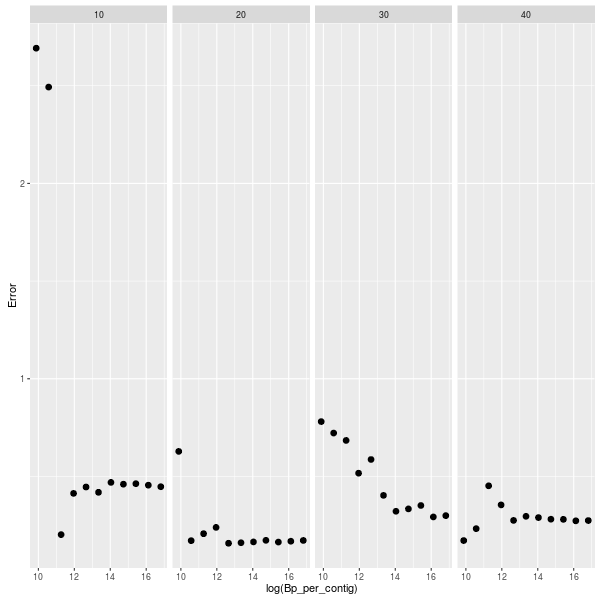
\includegraphics[width=.7\linewidth]{figures/fauxHumanErrorVsBpWithIntGrid.png}
  \caption{Relationship between error and bp per contig, split by different PSMC intervals for ``fauxHuman'' simulation.}\label{fauxHumanErrorVsBpWithIntGrid}
\end{figure}

For the steppe bison, there was an unusual trend when splitting the data (see Figure \ref{steppeBisonWeirdTrend}). The general trend was decreasing error as mean bp per contig was increased. However, there was an unusual drop in error for the splits of $2^8$ and $2^9$. This could possibly be due to error in scripting, but this is unlikely since all the runs were automated. It could also just be coincidence, and it would be interesting to see if this trend was replicated for different animals' genomes.

\begin{figure}[h]
  \center
  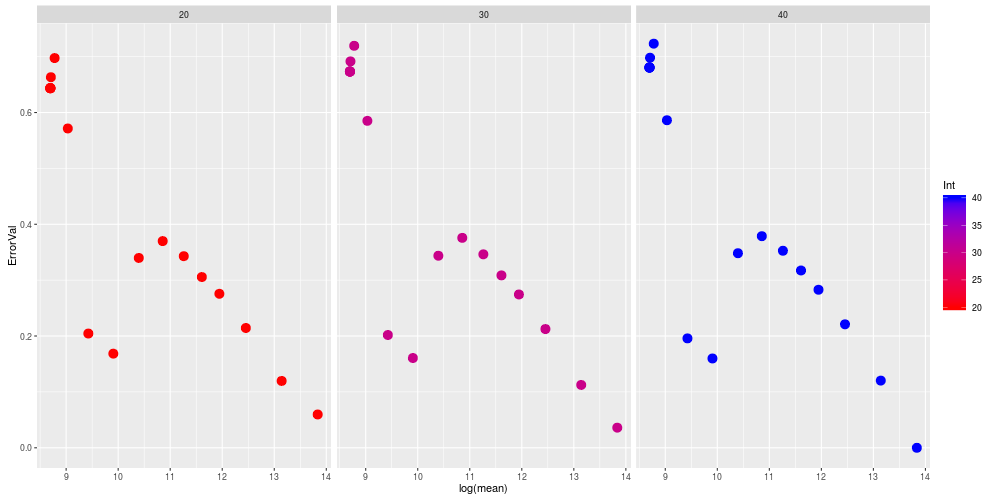
\includegraphics[width=.7\linewidth]{figures/steppeBisonWeirdTrend.png}
  \caption{Relationship between error and log mean bp per contig for steppe bison data.}\label{steppeBisonWeirdTrend}
\end{figure}

\subsection{Deleting Data}
Analysis of the deleting data experiment using the R script \verb|sim2PartAnalysis.R| yielded the PSMC plots Figure \ref{deletedDataPsmcPlots} (showing the different population estimates) and Figure \ref{sim2ErrorVsMeanContigLength} (showing the error for different mean contig lengths). Figure \ref{sim2ErrorVsMeanContigLength} was found to give a well-fitted straight line if a log transform was applied to the mean contig length.

It was suggested that a better alternative to randomly deleting lines would be to randomly replace lines with missing data (\verb|N| in the \verb|.psmcfa| file type). This would be representative of a low quality genome, and would allow comparison of error between a full genome and a genome with missing data.

It may be possible to construct a predictor for error based upon the amount of missing data, but this would be based upon extrapolation, so would be dangerous.

\begin{figure}[h]
  \center
  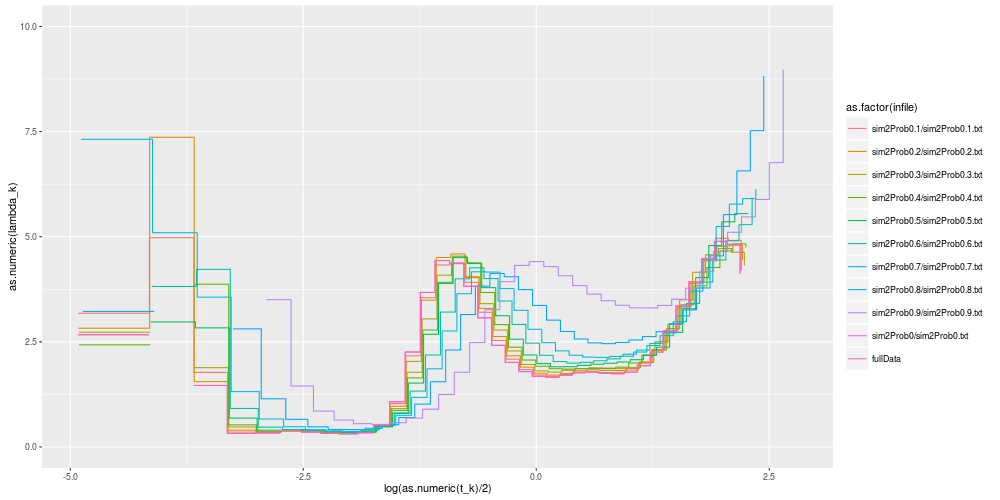
\includegraphics[width=1\linewidth]{figures/deletedDataPsmcPlots.png}
  \caption{The output from PSMC for various amounts of deleted simulated data.}\label{deletedDataPsmcPlots}
\end{figure}

\begin{figure}[h]
  \center
  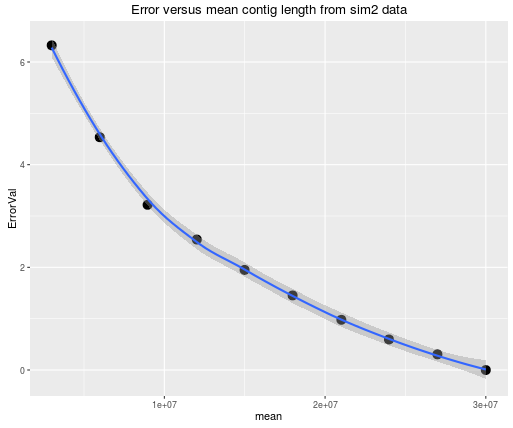
\includegraphics[width=.7\linewidth]{figures/sim2ErrorVsMeanContigLength.png}
  \caption{Relationship between error and mean contig length.}\label{sim2ErrorVsMeanContigLength}
\end{figure}

\subsubsection{Time Intervals}
Be careful of what intervals you use - if the resolution is too low, it can look like there is a sharp population decrease when it is actually gradual.

\subsection{Statistical Analysis of Error}
To get an idea of the relationships between variables, a multiple regression model was fitted first (see \verb|MixedEffNew160128.R|). Output from the best:
\begin{lstlisting}
> model = lm(formula = Error ~ Bp + Int + Pop_Dynamics_Type + lBpPC + Bp:Int + Bp:Pop_Dynamics_Type + Bp:lBpPC + Int:Pop_Dynamics_Type,  data = data)
> summary(model)

Call:
lm(formula = Error ~ Bp + Int + Pop_Dynamics_Type + lBpPC + Bp:Int + 
    Bp:Pop_Dynamics_Type + Bp:lBpPC + Int:Pop_Dynamics_Type, 
    data = data)

Residuals:
     Min       1Q   Median       3Q      Max 
-1.55701 -0.34754 -0.00454  0.20423  2.84862 

Coefficients:
                                Estimate Std. Error t value Pr(>|t|)    
(Intercept)                    0.9213000  0.4610826   1.998 0.046449 *  
Bp                             0.0658496  0.0345613   1.905 0.057531 .  
Int                           -0.0126008  0.0076566  -1.646 0.100685    
Pop_Dynamics_TypepsmcSim1      0.0561441  0.2458618   0.228 0.819498    
Pop_Dynamics_Typetrench        0.8183133  0.2959402   2.765 0.005981 ** 
lBpPC                          0.0484409  0.0326705   1.483 0.139019    
Bp:Int                        -0.0012719  0.0004937  -2.576 0.010381 *  
Bp:Pop_Dynamics_TypepsmcSim1  -0.0450938  0.0127914  -3.525 0.000477 ***
Bp:Pop_Dynamics_Typetrench     0.0419082  0.0139419   3.006 0.002832 ** 
Bp:lBpPC                      -0.0055009  0.0024187  -2.274 0.023528 *  
Int:Pop_Dynamics_TypepsmcSim1  0.0451173  0.0071347   6.324 7.51e-10 ***
Int:Pop_Dynamics_Typetrench    0.0315472  0.0076636   4.117 4.76e-05 ***
---
Signif. codes:  0 ‘***’ 0.001 ‘**’ 0.01 ‘*’ 0.05 ‘.’ 0.1 ‘ ’ 1

Residual standard error: 0.648 on 363 degrees of freedom
Multiple R-squared:  0.6945,	Adjusted R-squared:  0.6852 
F-statistic:    75 on 11 and 363 DF,  p-value: < 2.2e-16
\end{lstlisting}
On the basis of this, various mixed effects models were fitted. Output from the best:
\begin{lstlisting}
> summary(M4s)
Linear mixed model fit by REML ['lmerMod']
Formula: RtError ~ Bp + Int + lBpPC + Bp:Int + Bp:lBpPC + (1 + Bp + Int |      Pop_Dynamics_Type)
   Data: data_s

REML criterion at convergence: 138.4

Scaled residuals: 
    Min      1Q  Median      3Q     Max 
-2.6295 -0.5008 -0.0074  0.4045  3.4304 

Random effects:
 Groups            Name        Variance Std.Dev. Corr       
 Pop_Dynamics_Type (Intercept) 0.21281  0.4613              
                   Bp          0.01146  0.1070    0.78      
                   Int         0.01204  0.1097    0.61 -0.03
 Residual                      0.07369  0.2715              
Number of obs: 375, groups:  Pop_Dynamics_Type, 3

Fixed effects:
            Estimate Std. Error t value
(Intercept)  1.21144    0.26673   4.542
Bp          -0.10197    0.06349  -1.606
Int         -0.01607    0.06490  -0.248
lBpPC       -0.02340    0.01448  -1.616
Bp:Int      -0.03784    0.01411  -2.682
Bp:lBpPC    -0.03682    0.01429  -2.577

Correlation of Fixed Effects:
         (Intr) Bp     Int    lBpPC  Bp:Int
Bp        0.753                            
Int       0.593 -0.026                     
lBpPC     0.000 -0.056 -0.001              
Bp:Int    0.003 -0.004 -0.001  0.004       
Bp:lBpPC -0.013 -0.010  0.000  0.014  0.002
\end{lstlisting}

As the number of base pairs in a sample creates a lot of variance and we were examining small (Mbp) levels compared with genomes (Gbp), we decided to only use the largest sample size, 20 Mbp. It probably would have been a better idea to use Gbp size genomes for testing (this would take longer, obviously).

Multiple regression is a decent starting point, however as some of the data points originate from the same genome, the assumption of independence is violated. Additionally, some of the diagnostic plots looked dodgy (see assumption checking in \verb|MixedEffNew160128.R|).

Next, mixed effects modelling was used. We allowed different intercepts to vary with the different type of population dynamics. On the basis of AIC, the best model was selected. However some of the diagnostic plots also looked off.

Still working towards finding a reliable method of predicting error. The main factor affecting error prediction appears to be the population dynamics.

A limitation of this error technique is that it doesn't give an estimate of variance in population dynamics at points of interest.

\subsection{Misordering Data}
We didn't actually do this. But it would be interesting to see how much the error changes if things e.g. sequences in the contigs are put in the wrong order, or assembled wrong. Could do this randomly shuffling lines.
%\begin{itemize}
%\item Take \verb|.psmcfa| file.
%\item Re-order contigs (e.g. the first contig swaps with the second contig). This will n%ot yet change the results of PSMC.
%\item Combine all the contigs into one giant chromosome using \verb|combinePsmcfa.sh|.
%\item Using something like \verb|binarySplitPsmcfaPrint.py| or a similar script, break up the large chromosome. This will generate new contigs.
%\end{itemize}

\subsection{Checking the Model}

\subsubsection{Goodness of Fit}
Li \cite{li2011inference} has devised methods for checking goodness of fit, but I don't understand how to test this. In Section 2.2 of the Supplementary Information, he gives detail. There does not appear to be a script for extracting the statistics though.

In the S.I., Li says that you can check $C_\sigma\pi_k$ for overfitting. If it's small (e.g. less than 20), you shouldn't trust the estimates of $\lambda_k$. I'm not sure how to get this value though.
\subsubsection{Correcting for False Negatives}
In Appendix II of the PSMC README file, Li talks about correcting for false negatives in the case of low coverage (for example, the kangaroo only had 55\% coverage). I'm not sure how to estimate this, you should probably talk to a biologist.


\section{Kangaroo Analysis}
\subsection{Data Processing}
Using a tammar wallaby reference genome (\url{acad-colab1@acad2.rc.adelaide.edu.au:/localscratch/Refs/Macropus_eugenii/Meug_1_0_Raw/Macropus_eugenii.Meug_1.0.dna_rm.toplevel.fast}), the kangaroo genome was aligned, giving a \verb|.bam| file (\url{acad-colab1@acad2.rc.adelaide.edu.au:/localscratch/AussieGenomes/Kangaroo/bwa_n0.04_seed/Kangaroo.Meug_1_0.realigned.bam}).

The overall depth was $3.9\times$, but given there were many missing values due to the reads covering only 55\% of the wallaby genome, the overall depth for bases read at least once was $7.2\times$. This was found by the following code.
\begin{lstlisting}
# Depth
samtools depth Kangaroo.Meug_1_0.realigned.bam > Kangaroo.Meug_1_0.realigned.depth
# Genome size from bam file (to use instead of "NR" in previous command to get 'true' coverage)
samtools view -H Kangaroo.Meug_1_0.realigned.bam | grep -P '^@SQ' | cut -f 3 -d ':' | awk '{sum+=$1} END {print sum}'
# 2955773937
# Coverage
wc -l Kangaroo.Meug_1_0.realigned.depth
# 1626674725
# = 55.0% of genome (2955773937)
# mean depth
# for number of bases covered at least once (!!!)
samtools depth Kangaroo.Meug_1_0.realigned.bam | awk '{sum+=$3; sumsq+=$3*$3} END { print "Average = ",sum/NR; print "Stdev = ",sqrt(sumsq/NR - (sum/NR)**2)}'
# Average =  7.15569
# Stdev =  23.6263
# for all bases (use genome size instead of "NR" in previous command to compute 'true' coverage)
samtools depth Kangaroo.Meug_1_0.realigned.bam |  awk '{sum+=$3; sumsq+=$3*$3} END { print "Average = ",sum/2955773937; print "Stdev = ",sqrt(sumsq/2955773937 - (sum/2955773937)**2)}'
# Average =  3.93805
# Stdev =  17.885
\end{lstlisting}

A pseudo-diploid sequence in the FASTQ format was generated by the following commands.
\begin{lstlisting}
samtools mpileup -EA -Q20 -C50 -u -f Macropus_eugenii.Meug_1.0.dna_rm.toplevel.fasta Kangaroo.Meug_1_0.realigned.bam | bcftools call -c | vcfutils.pl vcf2fq | gzip > mpileupedKangaroo.fq.gz
\end{lstlisting}

This was converted into the \verb|.psmcfa| PSMC input format via the following command.
\begin{lstlisting}
fq2psmcfa redKangaroo.fq.gz > redKangaroo.psmcfa
\end{lstlisting}
PSMC was run, and population data was extracted.
\begin{lstlisting}
psmc redKangaroo.psmcfa > redKangarooInt4+5\*3+4.psmc
/home/alex/Desktop/Data/shaunWork/myScripts/removeDataFromPSMC.sh redKangarooInt4+5\*3+4.psmc > redKangarooInt4+5\*3+4.txt
\end{lstlisting}
\subsection{Analysis}
Rescaling and analysis were carried out in R (see \verb|redKangarooRPlots.R|).

\section{Tasmanian Devil Analysis}
Carried out in the same way as the red kangaroo. See \verb|tasmanianDevilRPlots.R|. The plots I showed to ACAD 

\bibliographystyle{plain}
\bibliography{MyBibliography}{}
\newpage

\appendix
\section{List of scripts}
\subsection{alexScripts}
These are the Alex's files which are worth looking at.
\begin{table}[h]
\begin{tabular}{p{6.5cm}p{8.5cm}}
  \hline
  \textbf{Name} & \textbf{Description} \\ 
  \hline
\parbox[t]{5cm}{\texttt{PSMC\_Regression/}\\ \texttt{StringExtraction\_ErrorAnalysis.R}} & Extracts information about the genome and PSMC run, does an error analysis, and outputs to text files. Designed for use with ms simulations, but can be adapted to be used with real data.\\ \hline
  \parbox[t]{5cm}{\texttt{PSMC\_Regression/}\\ \texttt{MixedEffNew160128.R}} & Attempt at fitting multiple regression, and then mixed effects model to various simulated genomes. It wasn't successful in producing a good model. There may be some dodgy things here, like failing independence assumptions, and using a Box-Cox transform for a mixed effects model (?). \\ \hline
  \parbox[t]{5cm}{\texttt{redKangaroo/}\\ \texttt{redKangarooRPlots.R}} & Plots various PSMC runs of the red kangaroo dataset. Also includes ice age start and end. \\ \hline
  \parbox[t]{5cm}{\texttt{tasmanianDevil/}\\ \texttt{tasmanianDevilRPlots.R}} & Plots various PSMC runs of the Tasmanian devil (and red kangaroo dataset). This is a better file than the red kangaroo R file. \\ \hline
  \texttt{diffPSMCInts.sh} & A modified version of Shaun's \verb|runDataCollection.sh| script, without the binary splitting. \\
  \texttt{Mixed Effects Test.R} & An example, following the instructions of Zuur (2009) on how to fit mixed effects models in R. \\
  \hline
\end{tabular}
\end{table}

\subsection{shaunScripts}
These scripts have short comments at the beginning, which gives some detail on what they do, and how to run them. You should look at the files themselves before attempting to run them. Paths to programs inside the scripts will probably have to be changed. I advise putting the directories with PSMC etc. in your bash \verb|.profile| file, so that you can just write \verb|psmc| instead of \verb|/path/to/file/psmc| every time.

All python scripts require python 3.
\begin{table}[h]
\begin{tabular}{p{6.5cm}p{8.5cm}}
  \hline
  \textbf{Name} & \textbf{Description} \\ 
  \hline
  \parbox[t]{5cm}{\texttt{genome2PSMC/}\\ \texttt{extendSplits.sh}} & Splits simulated data in a binary manner up to 131072. Use it if you've already done binary splits up to 1024.\\ \hline
  \parbox[t]{5cm}{\texttt{genome2PSMC/}\\ \texttt{pileupBAMFile.sh}} & Gets a \verb|.bam| file (genome) and a \verb|.fasta| file (reference) and matches them to produce a pseudo-diploid \verb|.fq.gz| file.\\ \hline
  \parbox[t]{5cm}{\texttt{genome2PSMC/}\\ \texttt{runDataCollection.sh}} & Runs PSMC with 4 different time intervals, does binary splitting up to 1024, takes summary statistics on the genome, extracts population dynamics in text files.\\ \hline  
  \texttt{binarySplitPsmcfaPrint.py} & Takes a \verb|.psmcfa| file and splits every contig/chromosome into two (with a floor of one line).\\ \hline  
  \texttt{misorderPsmcfa.py} & Unfinished script which is supposed to take a \verb|.psmcfa| shuffle lines about randomly.\\ \hline  
  \texttt{removeRandomContigs.py} & Removes contigs randomly from a \verb|.psmcfa| file.\\ \hline  
\texttt{removeRandomPartsFromPsmcfa.py} & Removes lines randomly from a \verb|.psmcfa| file.\\ \hline  
\texttt{reorderContigs.py} & Shuffles the order of contigs in a \verb|.psmcfa| file. On its own, this does not change the output of PSMC. \\ \hline
\texttt{splitFasta.py} & Splits a \verb|.fasta| file and creates a text file for every contig. I would strongly advise against this, splitting is much more efficient on a \verb|.psmcfa| file, and if you run this on something with a billion contigs...\\ \hline  
\texttt{splitMs.py} & Same as \verb|splitFasta.py| but for \verb|.ms| output.\\ \hline 
\texttt{summaryStatisticsPsmcfa.py} & Gives tab delimited table of the minimum, maximum, mean, median and total length of all the contigs in a \verb|.psmcfa| file. \\ \hline
\texttt{growthDataSlidingWindowError.R} & Does a sliding window-style error analysis. \\ \hline
\texttt{steppeBisonPartAnalysis.R} & Looks at what happens to error if you remove parts of the steppe bison genome. \\ \hline
\texttt{steppeBisonSplitAnalysis.R} & Looks at what happens to error if you perform binary splitting the steppe bison genome. \\ \hline
\texttt{combinePsmcfa.sh} & Combines all contigs in a \verb|.psmcfa| file to create one giant contig! \\ \hline
\texttt{manyMs2Psmcfa.sh} & Converts all \verb|.ms| files in the directory to \verb|.psmcfa| files. \\ \hline
\texttt{manyPsmc2Plot.sh} & Produces plots from all \verb|.psmc| files in the directory using the util \verb|psmc_plot.pl|. We usually used R to make plots though. \\ \hline
\texttt{manyPsmcfa2psmc.sh} & Runs PSMC with 10 time intervals on all \verb|.psmcfa| files in the directory. \\ \hline
\texttt{ms2plots.sh} & Combines the above three scripts. \\ \hline
\texttt{partRemovalRepeated.sh} & Removes 10, 20, 30, ... , 90\% of a \verb|.psmcfa| file. \\ \hline
\texttt{removeDataFromPSMC.sh} & Takes population dynamics and relevant times from the last iteration in the PSMC process. Probably something that needs to be added is also taking PSMC's estimate of $\theta_0$ (the second number on the \verb|TR| line, take from the last iteration.)\\ \hline
\texttt{runSimulations.sh} & For a given set of population dynamics (specified in-file), will run ms with varying genome sizes, covert to \verb|.psmcfa|, perform PSMC with different time intervals, and extract the estimates of population dynamics. \\ \hline
\end{tabular}
\end{table}

\section{Data}
\begin{itemize}
\item The \verb|.psmcfa| files for the wood bison (we didn't analyse this), steppe bison, Tasmanian devil and red kangaroo can be found in the \verb|psmcfa| folder. Ask ACAD if you want the BAM and reference FASTA files, it's on their server.
\item Various simulation parameters can be found in the \verb|msParameters folder|. Note though that the ``constantPop'' and ``decreasing'' simulations did not give very useful results.
\item PSMC output for the Tasmanian devil and red kangaroo can be found in the \verb|data| folder. It's a bit of a mess in there, but you should be able to find the relevant files.
\item Scripts and R files can be found in the \verb|alexScripts| and \verb|shaunScripts| folders. Again, sorry for the mess, especially in the \verb|alexScripts| folder there is a lot of useless stuff.
\item Report-related material can be found in the \verb|reports| folder.
\item A copy of the PSMC paper, the S.I., and Hudson's ms manual is included in the \verb|papers| folder.
\end{itemize}


\end{document}
